% =============================================================
%  Chapter 5 — Evaluation
% =============================================================
%  Grounded in the final results/ snapshot (2026-07-31): 63 of a
%  possible 63 cells (7 scenarios x 3 frameworks x 3 models), full
%  coverage. Figures/tables regenerated by
%  scripts/analysis/aggregate_evaluation.py, which writes
%  results_aggregate/{cells,iterations,failures}.csv and
%  results_aggregate/figures/*.pdf, mirrored into figures/eval/ for
%  this chapter. Re-run that script and re-derive every number below
%  from the CSVs before editing this chapter by hand.
% =============================================================

\chapter{Evaluation}
\label{ch:results}

Chapter~\ref{ch:setup} fixed what was run: three models, seven scenarios,
three frameworks, one sample per cell. This chapter asks what it shows.
Rather than walking through every cell one at a time, it is organised
around seven research questions that each aggregate across every cell,
model, and scenario collected, closing with a synthesis that draws the
seven answers together and connects them back to the thesis's central
question (Section~\ref{sec:intro-missing}): \emph{can an LLM agent
iteratively optimise the deployment configuration of a backend application
on a Kubernetes cluster, guided by runtime performance feedback, to
maximise sustainable throughput under fixed infrastructure constraints?}

We achieved complete experiment coverage: all 63 of 63 cells spanning
these scenarios, frameworks, and models were evaluated, and every cell
reached a working baseline deployment and completed the full
ten-iteration refinement budget.


% ----- §5.1 Overview -----
\section{Overview of the Collected Data}
\label{sec:results-overview}

This section reports on \textbf{63 experiments} across the three models,
seven scenarios, and three frameworks introduced in
Chapter~\ref{ch:setup}. Each experiment records its per-iteration
goodput, the refinement lever applied, the resulting deployment-spec
knobs, and any failures observed; these records feed the figures and
summary statistics presented later in this chapter.

Every cell in this chapter reflects a single run, generated from one
code-generation and deployment-generation seed
(Section~\ref{sec:setup-procedure}); Section~\ref{sec:methods-metrics}
gives the rationale for this design and what it does and does not
support. Goodput and gain,
introduced from Section~\ref{sec:results-rq1} onward, are positive,
multiplicative quantities and are summarised using geometric means.
Individual scenario-level points are shown alongside every aggregate so
the reader can assess variation directly rather than rely on a single
summary statistic. Section~\ref{sec:discussion-limitations} discusses in
more detail what this single-run design does and does not allow us to
claim.


% ----- §5.2 RQ1 -----
\section{RQ1: Does Iterative Refinement Improve Sustained Goodput?}
\label{sec:results-rq1}

\begin{table}[htbp]
  \centering
  \caption{First-non-zero-goodput vs.\ best-iteration goodput, by model,
    as geometric means over cells with positive goodput ($n$ valid, out
    of 21). \emph{Healthy baseline} is the stricter count of cells already
    serving traffic at iteration \texttt{000}. \emph{Gain} is the
    geometric mean of each cell's own best/first-non-zero ratio.}
  \label{tab:results-rq1-summary}
  \small
  \begin{tabular}{@{}lrrrrr@{}}
    \toprule
    \textbf{Model} & $n$ valid & Healthy baseline & First non-zero & Best & Gain \\
    \midrule
    \texttt{claude-opus-4-8} & 20 / 21          & 12 / 21          & 4{,}084           & 13{,}382          & $\mathbf{3.3\times}$ \\
    \texttt{gpt-5.5}         & \textbf{21 / 21} & \textbf{15 / 21} & \textbf{11{,}989} & \textbf{32{,}817} & $2.7\times$ \\
    \texttt{glm-5.2}         & 20 / 21          & 7 / 21           & 4{,}952           & 12{,}630          & $2.5\times$ \\
    \bottomrule
  \end{tabular}
\end{table}

\paragraph{Evidence.}
Table~\ref{tab:results-rq1-summary} aggregates all 63 cells by model: for
each cell it compares the first iteration with positive goodput against
that cell's own best iteration, and reports the geometric-mean ratio
between them as the \emph{gain}. Figure~\ref{fig:results-baseline-vs-best}
(below) shows the first-vs-best comparison aggregated per model, with
every cell's own value plotted alongside the geometric mean.
Figure~\ref{fig:results-trajectories-grid} (further below) shows the same
63 trajectories individually, one panel per scenario$\times$framework
cell. Cells that never record positive goodput at any iteration have no
valid gain reference and are excluded from these geometric means rather
than counted at $0$ (the table's ``$n$ valid'' column). The same two
cells appear in Figure~\ref{fig:results-trajectories-grid} as panels
whose trajectory never leaves zero across all ten iterations.

\texttt{gpt-5.5} leads on both ends, and not by a small margin: its
geometric-mean best ($32{,}817$\,req/s) is more than double
\texttt{claude-opus-4-8}'s ($13{,}382$) and roughly $2.6\times$
\texttt{glm-5.2}'s ($12{,}630$). It also has the highest first-non-zero
goodput and the most cells with an already-healthy baseline (15 of 21),
meaning it most often produces a baseline strong enough to go straight
into refinement rather than needing to recover from a dead start first.

\texttt{glm-5.2} sits at the other end on the healthy-baseline measure,
with the fewest healthy baselines of the three (7 of 21, less than half
of \texttt{gpt-5.5}'s 15), yet still reaches a geometric-mean best
goodput ($12{,}630$\,req/s) close to \texttt{claude-opus-4-8}'s
($13{,}382$): whatever state the baseline is in, refinement closes most
of the gap by the best iteration.

\texttt{claude-opus-4-8} shows the largest geometric-mean gain of the
three ($3.3\times$), largely because it also starts from the lowest
first-non-zero goodput. The same absolute improvement reads as a larger
multiplicative gain from a lower starting point, so this result says more
about where its trajectories start than about how strong its best
iteration is. Its geometric-mean best ($13{,}382$\,req/s) sits well below
\texttt{gpt-5.5}'s but only modestly above \texttt{glm-5.2}'s
($12{,}630$). Section~\ref{sec:results-rq5} traces this shortfall to a
pair of low-goodput \textsc{Rust-Actix} cells that stall at their first
successful iteration, not to a general weakness of that framework for
\texttt{claude-opus-4-8}.

\begin{figure}[htbp]
  \centering
  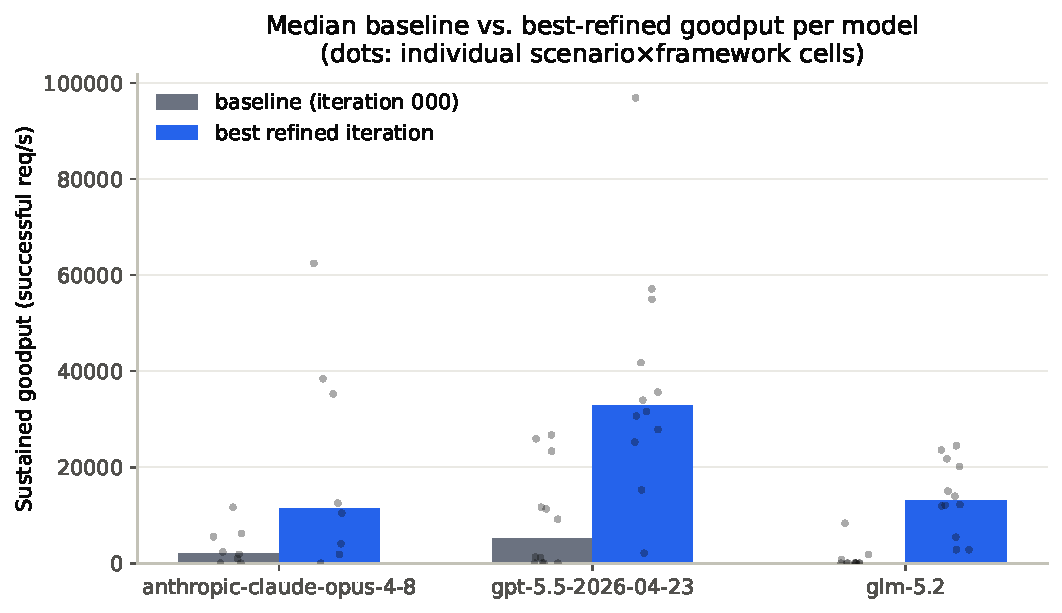
\includegraphics[width=0.85\linewidth]{figures/eval/baseline_vs_best_by_model.pdf}
  \caption{First-non-zero-goodput vs.\ best-refined-iteration goodput, per
    model. Boxes show the quartiles and full range across cells with
    positive goodput; diamonds mark the geometric mean reported in the
    text and Table~\ref{tab:results-rq1-summary}; dots show every
    individual cell (one scenario$\times$framework combination per model).}
  \label{fig:results-baseline-vs-best}
\end{figure}

Figure~\ref{fig:results-baseline-vs-best} and Table~\ref{tab:results-rq1-summary}
make the same point from two directions. \texttt{gpt-5.5}'s first-non-zero
geometric mean ($11{,}989$\,req/s) is on par with \texttt{glm-5.2}'s and
\texttt{claude-opus-4-8}'s \emph{best}-iteration geometric means
($12{,}630$ and $13{,}382$\,req/s): on average, its baseline already
reaches the goodput level the other two models only reach after
refinement. This is not an average pulled up by a handful of strong
cells: \texttt{gpt-5.5}'s whole first-non-zero box sits close to the
other two models' best-iteration boxes, not just its geometric mean, and
even its lowest first-non-zero value ($1{,}182$\,req/s) is higher than
either other model's lowest. The boxes also differ in width:
\texttt{claude-opus-4-8} has the widest spread of the three models on
both the first-non-zero and best-iteration side, driven by the same low
outliers noted above. \texttt{glm-5.2}'s best-iteration box is the
narrowest of the three, its refined cells landing in a comparatively
tight band regardless of how healthy the baseline was.

\FloatBarrier
\begin{figure}[htbp]
  \centering
  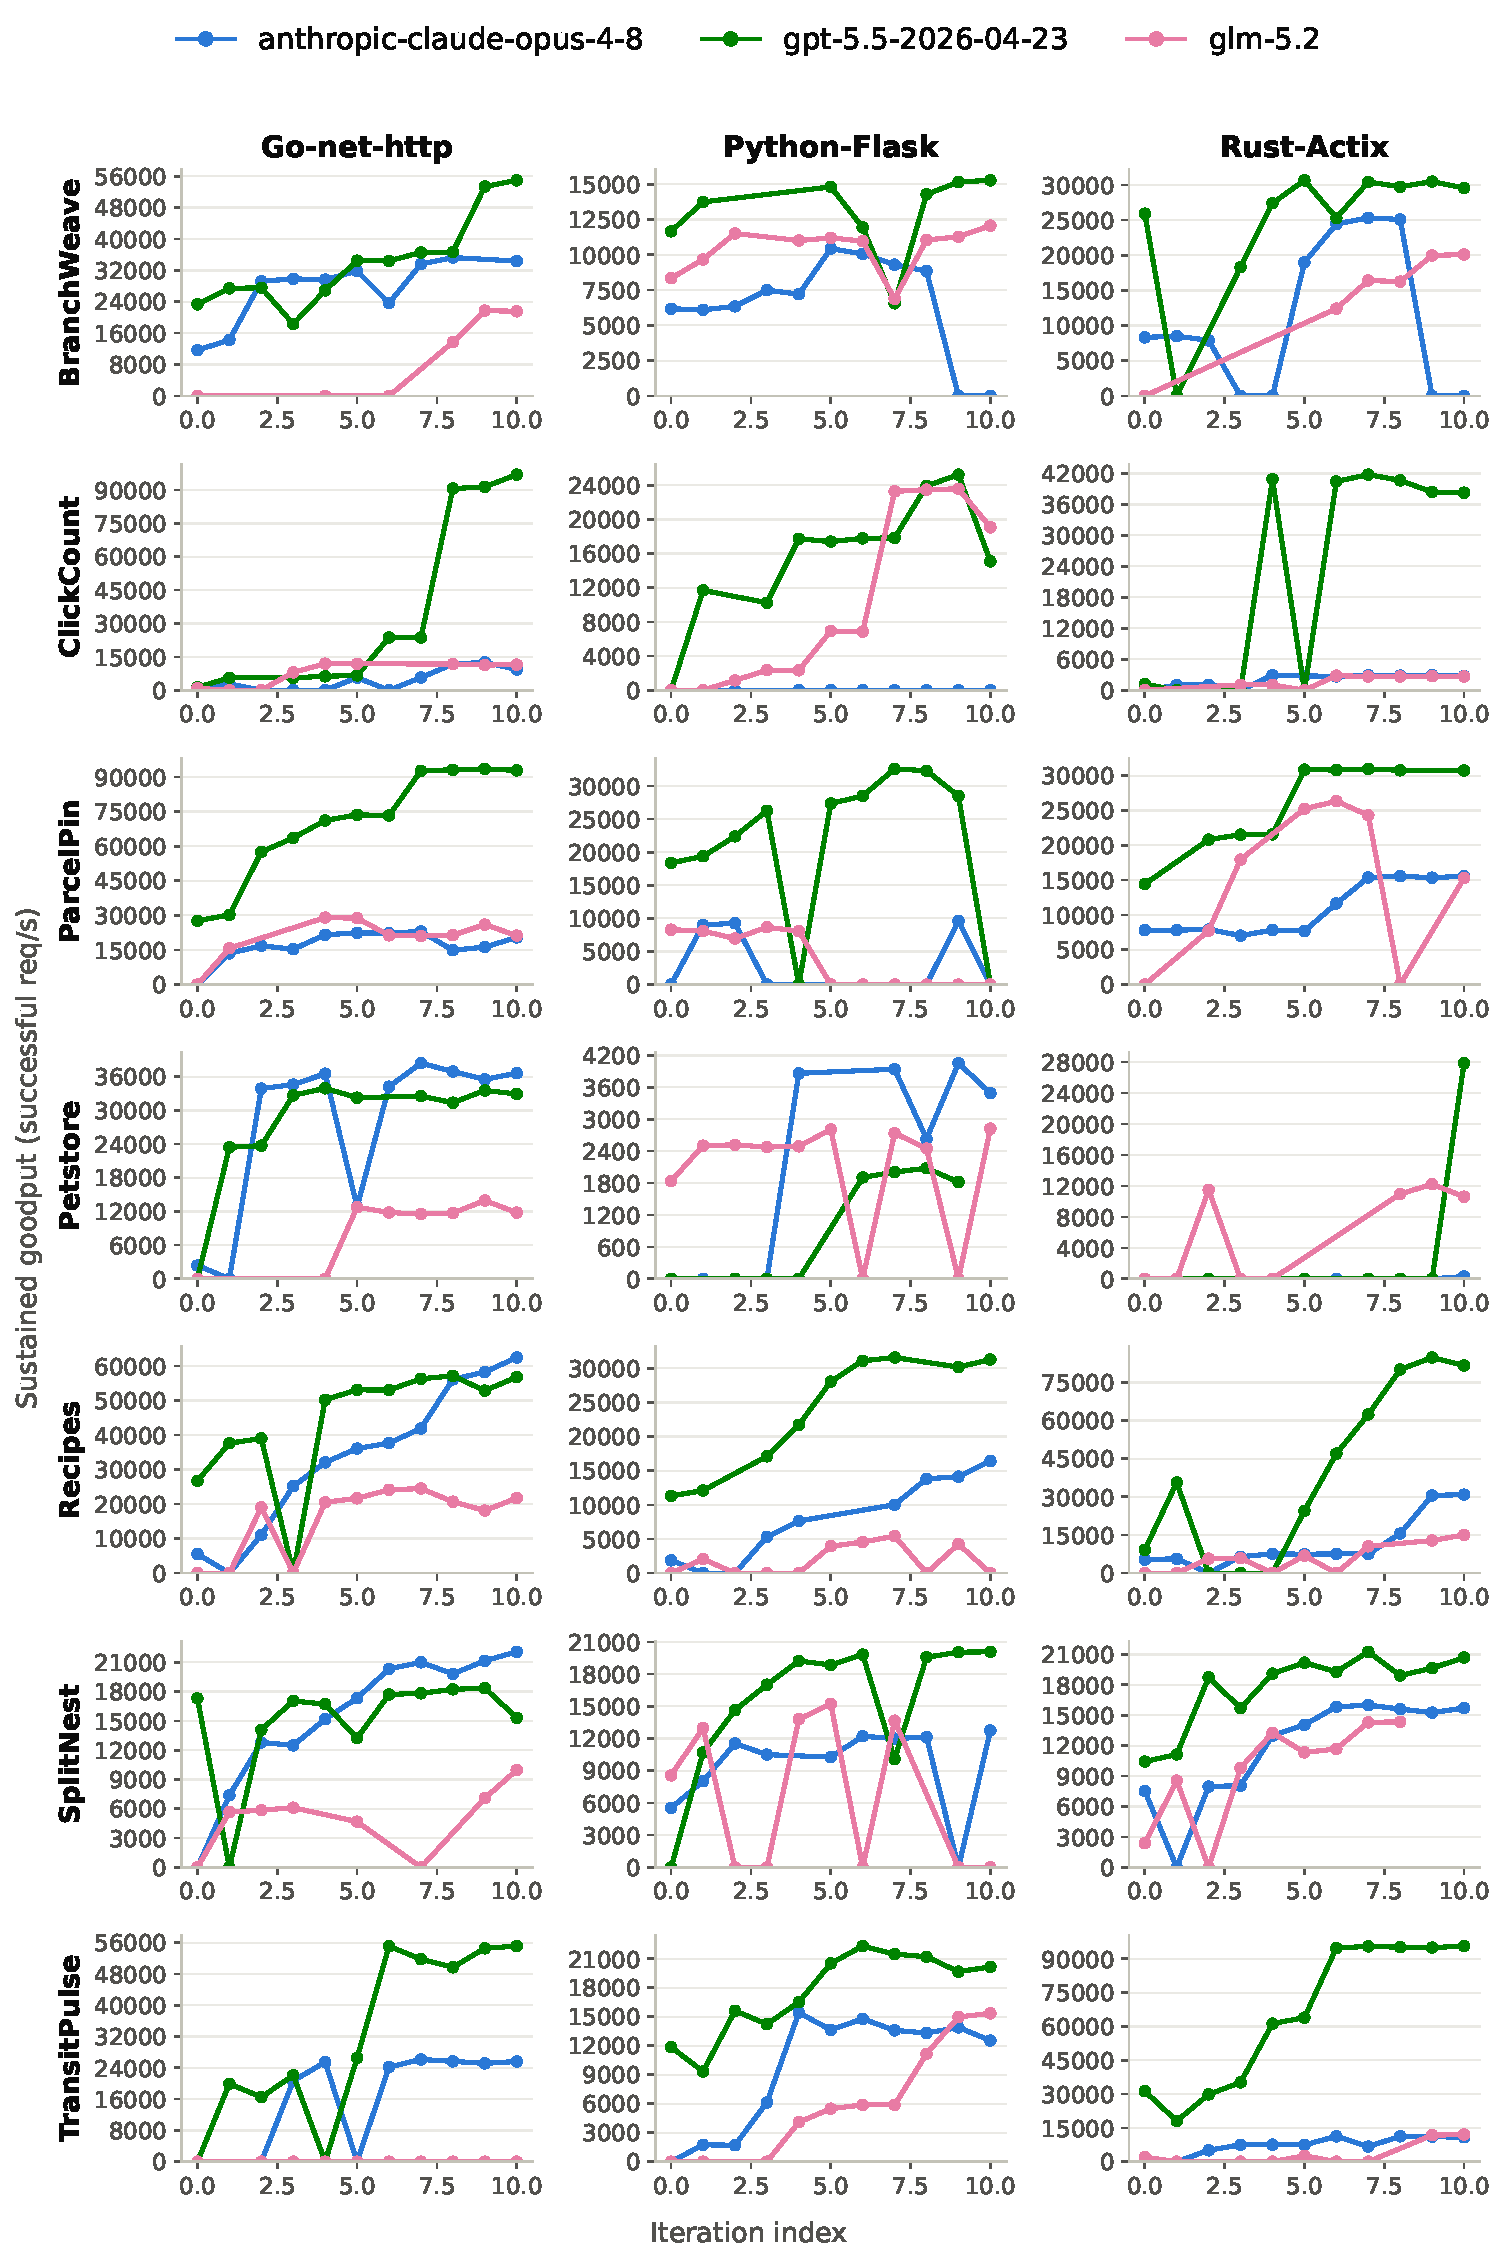
\includegraphics[width=1\linewidth]{figures/eval/goodput_trajectories_grid.pdf}
  \caption{Sustained goodput per iteration, one panel per
    scenario$\times$framework combination, coloured by model; note the
    independent $y$-axis per panel.}
  \label{fig:results-trajectories-grid}
\end{figure}
\FloatBarrier

\newpage
\paragraph{Refinement also rescues \emph{dead} baselines, almost always.}
Figure~\ref{fig:results-trajectories-grid} plots the sustained goodput
recorded at each refinement iteration, not the higher load levels
explore deliberately probes to find where the deployment collapses
(Section~\ref{sec:methods-load-profile}). A trajectory that stays at
$0$\,req/s therefore means the deployment failed one of the health gates
guarding refinement, the warm-up check, recovery, or the per-level
failure-rate check inside refine, not necessarily that it could serve no
requests at any load. Across all three models,
\textbf{29 of the 63 cells} start with an unhealthy baseline, and
\textbf{27 of those 29} recover to a non-zero deployment somewhere in
their trajectory: all 6 of \texttt{gpt-5.5}'s dead baselines recover, 13
of \texttt{glm-5.2}'s 14 dead baselines recover, and 8 of
\texttt{claude-opus-4-8}'s 9 dead baselines recover. Two cells never
recover across the full ten-iteration budget: \texttt{claude-opus-4-8}'s
\textsc{ClickCount}$\times$\textsc{Python-Flask} and \texttt{glm-5.2}'s
\textsc{TransitPulseDelayReporter}$\times$\textsc{Go-net-http}, the latter
recording exactly $0$\,req/s at every one of its ten iterations despite the
decision stage trying both code and deployment refinement across the
trajectory. Refinement therefore contributes more than a tuning-speed
improvement: in most of these cases it brings a deployment that was not
clearing our health gate up to an accepted sustained-goodput level under
our load profile, though, as the two non-recovering cases show, recovery
is not guaranteed.

\paragraph{Improvement is not perfectly monotonic and can end in failure.}
Individual iterations often regress relative to the preceding successful
iteration, producing the sawtooth patterns in
Figure~\ref{fig:results-trajectories-grid}. Because the framework
updates the trajectory's latest \emph{successful}-benchmark reference
only after a completed run (Section~\ref{sec:methods-outcome}),
regressions are not silently
compounded: the next decision stage receives them as feedback, and most
trajectories recover within one or two iterations.
\textsc{BranchWeave}$\times$\textsc{Rust-Actix} on \texttt{claude-opus-4-8}
is the sharpest exception. After reaching $25{,}327.3$\,req/s at
iteration~007, two consecutive spec-refinement iterations, 009, which
reduced database replicas from 3 to 2, and 010, which reduced
\texttt{max\_connections} from 400 to 250, drove goodput to zero. The
trajectory then exhausted its budget, ending at $0$\,req/s despite having
reached $3\times$ its own baseline just one iteration earlier. Unlike the
dead baselines above, this cell began healthy; it failed only at the end
of an otherwise successful trajectory, with no iterations remaining for
recovery. Section~\ref{sec:results-rq7} discusses a milder case that
recovers more slowly but before the budget is exhausted.

\paragraph{Interpretation.}
Iterative refinement improves sustained goodput in essentially every cell
with data, and the size of the multiplicative gain is dominated by how
badly under-provisioned the baseline happened to be (largest for both
models that show it on the same near-stateless scenario), which is closer
to a property of the baseline LLM call and the scenario's workload shape
than of the refinement loop itself. Two cells never recover from a dead
baseline regardless of which lever the decision stage tries, and a third,
distinct case shows the mirror-image risk: a cell that already recovered
and peaked well above baseline can still end its fixed budget at zero if
its last two decisions both regress it and nothing is left to try again.
Neither failure mode is attributable to a specific structural cause
without further trajectory-level instrumentation.

\paragraph{Conclusion.}
\textbf{Yes, with two caveats.} Refinement improves goodput in every model
whenever a cell has data, and in a large majority of cells (27 of 29) it is
not a marginal improvement but the difference between a non-functional and
a functional deployment. The size of the multiplicative gain is not a fixed
``refinement value-add'' comparable across cells: it tracks how
under-provisioned the baseline was, most sharply on the near-stateless
\textsc{ClickCount} scenario, for the two models where a large outlier
appears at all. Separately, a fixed iteration budget is not just a sample-size
limitation but a real risk: this dataset now contains a cell that ends at
zero goodput purely because its budget ran out one or two iterations before
it could recover from a late regression, the sharpest of a few cells whose
final iteration lands at zero despite an earlier healthy peak.


% ----- §5.3 RQ2 -----
\section{RQ2: Does the Load Profile Itself Locate Sustained Goodput
  Efficiently and Reliably?}
\label{sec:results-rq2}

Every goodput number in this chapter, RQ1's included, comes from a single
measurement instrument: the Explore-and-Refine load profile
(Section~\ref{sec:methods-load-profile}). Rather than being handed a target
rate, the profile searches for a deployment's sustainable throughput in four
phases: a health-gated warm-up, an aggressive explore ramp, a conservative
recovery step, and a fine-grained refine search. This question validates the
instrument rather than making a new claim about the systems it measures: if the
profile locates sustained goodput slowly, inconsistently, or only across a
narrow range of deployments, every other result in this chapter inherits that
weakness silently. We ask it in four parts: how much wall-clock time the search
costs, and where that time is spent across the four phases; how the refined
estimate the profile reports relates to the peak goodput the explore phase
observes on the way to it; how stable that estimate is when the same deployment
is measured twice; and how often the profile reaches a usable estimate at all,
given that it deliberately drives every deployment into overload at least once.

This question works one level below the rest of the chapter. Elsewhere,
iterations are compared by the single goodput number each reports; here we look
inside an individual bench run, at the four phases the profile passes through on
the way to that number. The analysis covers all 631 bench runs that reached the
bench stage, not only the 63 baseline runs, and is reconstructed entirely from
the diagnostics each run already recorded, so it required no additional
benchmarking.

\paragraph{Efficiency.}
Figure~\ref{fig:results-rq2-phase-durations} shows each phase's wall-clock
duration across all parsed runs. The warm-up gate is fixed at 30\,s by
construction. Explore is the dominant cost (median 246\,s, IQR 157--342\,s, up
to 588\,s), consistent with its being the phase that sweeps the widest range of
load levels. Recovery is cheap and usually settles on the first attempt (median
45\,s, IQR 45--46\,s, matching the profile's 45\,s settle window). Refine costs
less than explore despite being the more careful search (median 62\,s, IQR
41--105\,s), because its efficiency-scaled step size shrinks automatically as
the deployment nears its ceiling. A complete run takes a median of 402\,s (IQR
303--513\,s, maximum 1{,}154\,s), comfortably inside the profile's 30-minute
(1{,}800\,s) budget in every one of the 631 runs: the search consistently
terminates on its own phase-completion criteria, not because the time budget
forced it to stop.

\begin{figure}[htbp]
  \centering
  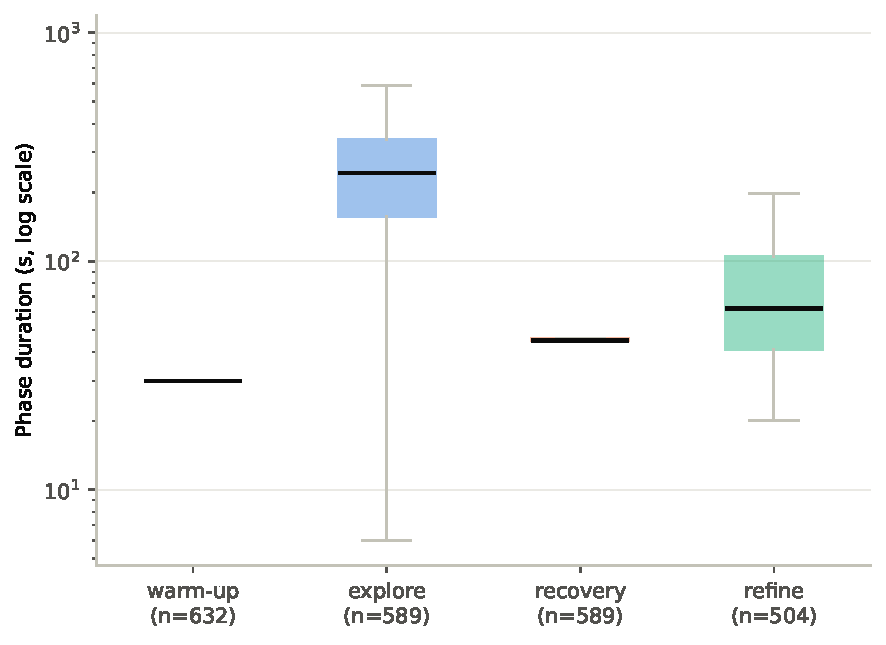
\includegraphics[width=0.72\linewidth]{figures/eval/load_profile_phase_durations.pdf}
  \caption{Wall-clock duration by load-profile phase, across all 631
    individual bench runs in this dataset (log scale; warm-up is
    effectively fixed at 30\,s by construction).}
  \label{fig:results-rq2-phase-durations}
\end{figure}

\paragraph{Accuracy.}
Restricted to the 479 runs that report a positive sustained-goodput estimate,
that estimate spans 287\,req/s to 96{,}925\,req/s, more than two orders of
magnitude, which is the range the exponential explore ramp is built for: a
linear staircase fine enough to resolve the low end would need an impractical
number of steps to reach the high end. Figure~\ref{fig:results-rq2-peak-vs-sustained}
compares, for each of these runs, the explore phase's recorded peak goodput
against refine's final sustained estimate. The usual pattern is the expected
one: refine settles below the transient explore peak (median gap $+8.4\%$, IQR
$0.2$--$33.9\%$), reflecting that a peak reached while still ramping upward is
not a level the deployment can hold indefinitely. Less expected, in $23.8\%$ of
runs the refined estimate is \emph{higher} than the explore peak. The clearest
instance is \texttt{gpt-5.5}'s \textsc{ClickCount}$\times$\textsc{Python-Flask},
iteration~5: explore stops at 8{,}750 users after a single p95 spike to
1{,}100\,ms (peak 6{,}817.7\,req/s), whereas refine's stability-gated search
from the recovered level climbs past that figure to settle at 18{,}560 users
and 17{,}401.2\,req/s, $2.55\times$ higher. Explore's fast, coarse ramp is
vulnerable to exactly this kind of transient latency spike; refine exists in
part to correct for it, not merely to trim a safety margin off a peak that was
already trustworthy.

\begin{figure}[htbp]
  \centering
  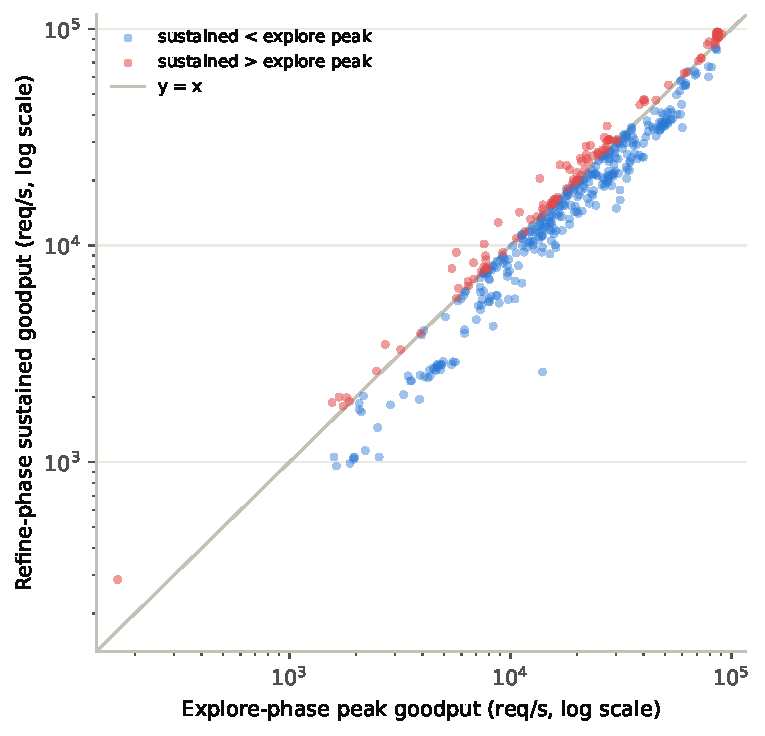
\includegraphics[width=0.62\linewidth]{figures/eval/load_profile_peak_vs_sustained.pdf}
  \caption{Explore-phase peak goodput vs.\ the refine-phase sustained
    estimate, one point per bench run with both quantities defined
    ($n=479$). Points above the $y=x$ line settle higher than their own
    recorded explore peak.}
  \label{fig:results-rq2-peak-vs-sustained}
\end{figure}

\paragraph{Repeatability.}
Accuracy so far concerns the profile's two internal estimates within a single
run; it says nothing about how stable the reported estimate is when the same
deployment is measured twice. To probe that, each fixed candidate was
re-measured in a deploy-only re-verification that repeats the benchmark without
changing the application code or its deployment. Across the candidates measured
in both runs, the estimate is typically very stable: the symmetric difference
between the two measurements has a median of $0\%$ and a mean of $7.1\%$, with
per-model medians of $3.4\%$ for \texttt{claude-opus-4-8}, $0.5\%$ for
\texttt{gpt-5.5}, and $0\%$ for \texttt{glm-5.2}.

This stability is not uniform across the study, and the reason is instructive.
Part-way through data collection, a network-path change moved the benchmark
traffic onto the isolated experiment LAN. Candidates measured before that change
repeat far less tightly than those measured after it: for the re-run candidates,
the median symmetric difference falls from $10.8\%$ before the change to $2.6\%$
after it, with the pre-change tail reaching several hundred percent on
individual candidates. The run-to-run noise this paragraph is meant to quantify
is therefore dominated by an environmental confound that was corrected during
the study rather than by the search strategy itself, which is a caveat on the
absolute goodput levels of the earliest runs. These figures are provisional in
one further respect: the re-verification does not yet cover every candidate, and
the pre-change runs were not themselves repeated, so the before/after contrast
is consistent with the network confound without isolating it as the sole cause.
Completing the re-verification set is what remains to settle the numbers.

\paragraph{Reliability and robustness.}
Table~\ref{tab:results-rq2-funnel} follows all 631 runs through the four gates
the profile must clear to report an estimate. $92.2\%$ survive the 30-second
warm-up health check, and every run that survives goes on to trigger one of
explore's stop conditions: roughly half on a latency breach ($49.5\%$), just
over a third on a goodput collapse ($37.3\%$), and the rest on a failure-rate
breach ($7.9\%$) or the 100{,}000-user ceiling ($5.3\%$). Of the runs that reach
it, recovery succeeds, and hands off to refine, in $86.6\%$ of cases. Refine in
turn produces a usable estimate in $95.0\%$ of the runs that reach it; the other
25 enter refine only to hit immediate overload before completing a single stable
settle window, so a successful recovery is not itself a guarantee that refine
will report a nonzero number. Chaining the four gates, $75.9\%$ of all 631 runs
produce a positive sustained-goodput estimate; the rest report exactly $0$,
through the same failure mechanisms RQ1 describes qualitatively
(Section~\ref{sec:results-rq1}): a warm-up that never passes, a recovery that
exhausts its retries, or a refine phase that overloads before settling a single
level. These are now counted precisely at the level of individual bench runs
rather than only the baseline iterations.

\begin{table}[htbp]
  \centering
  \caption{Phase-outcome funnel across all 631 bench runs.}
  \label{tab:results-rq2-funnel}
  \small
  \begin{tabular}{@{}lrr@{}}
    \toprule
    \textbf{Gate} & \textbf{Count} & \textbf{\% of previous stage} \\
    \midrule
    Total bench runs                   & 631 & --- \\
    Survives warm-up                   & 582 & $92.2\%$ \\
    Recovery succeeds                  & 504 & $86.6\%$ \\
    Refine produces an estimate        & 479 & $95.0\%$ \\
    \bottomrule
  \end{tabular}
\end{table}

None of these failure rates point to the profile being miscalibrated
toward excessive aggression: a $92.2\%$ warm-up survival rate leaves
comparatively few runs failing before the load profile has done anything
beyond holding a fixed, modest initial load, and the majority of the
remaining loss happens at recovery and refine, which is exactly where a
genuinely unhealthy or regressed deployment (Section~\ref{sec:results-rq1}'s
dead baselines and late regressions) would be expected to show up
regardless of which load profile measured it.

\paragraph{Interpretation.}
The profile costs a median of under seven minutes per run, well inside its
budget, and spends that time roughly where the mechanism design predicts: most
on the wide, aggressive explore search, least on the narrow, efficiency-gated
refine search. Its refined estimate is usually, but not always, below the
transient peak the explore phase observes, and the exception, refine settling
\emph{above} explore's peak in about a quarter of runs, is itself informative:
it shows that the coarse explore ramp can be fooled by a single latency spike
into stopping short of what a deployment can sustain, and that recovery and
refine do real corrective work rather than conservatively discounting a number
the profile already trusts. Three in four runs produce a usable estimate; of
those that do not, most fail at a stage (recovery or refine) that plausibly
reflects the deployment's own health rather than the search strategy.

\paragraph{Conclusion.}
\textbf{Yes, with repeatability still provisional.} The profile locates
sustained goodput efficiently, a median run costing under seven minutes and
never exhausting its budget, and it is robust enough to survive and recover from
the overload it deliberately induces in the large majority of runs ($86.6\%$
recovery success after an explore-stop, $75.9\%$ of all runs reaching a positive
estimate). Its refined estimate is not simply a discounted explore peak: it
settles below the peak when the peak was optimistic and above it when the peak
undersold the deployment. Where the same candidate has been re-measured, the
estimate is stable to within a few percent once the mid-study network confound
is accounted for; confirming that across the full re-verification set is the one
part of this question that remains open.


% ----- §5.4 RQ3 -----
\section{RQ3: Which Refinement Lever Contributes More: Code or Deployment?}
\label{sec:results-rq3}

\begin{figure}[htbp]
  \centering
  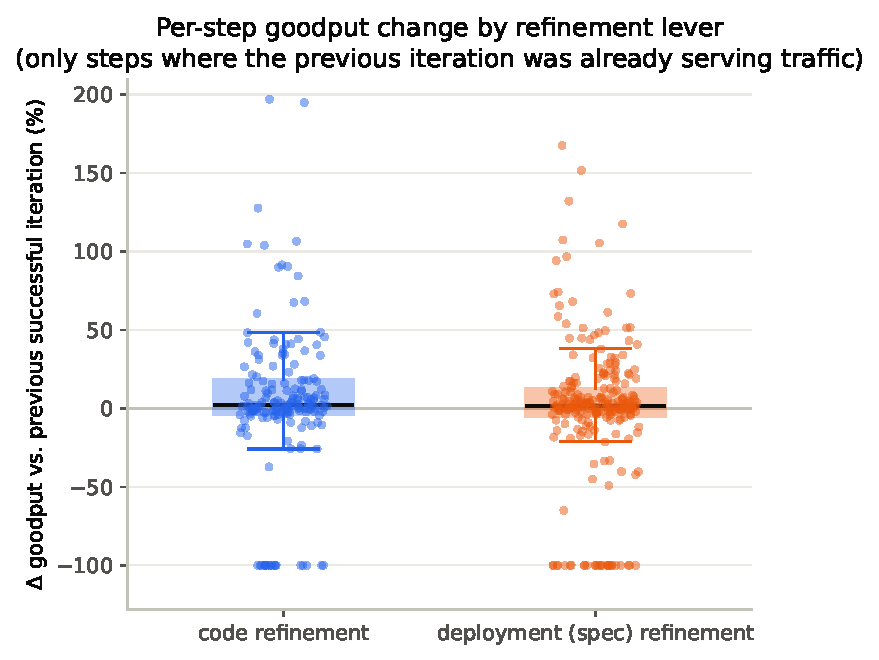
\includegraphics[width=0.75\linewidth]{figures/eval/code_vs_spec_delta.pdf}
  \caption{Per-step goodput change (\%) relative to the previous
    \emph{successful} iteration, split by refinement lever. Steps whose
    predecessor had zero sustained goodput are excluded here (their delta
    is undefined as a percentage) and discussed under RQ1/RQ7.}
  \label{fig:results-code-vs-spec}
\end{figure}

\paragraph{Evidence.}
Across all three models, 279 completed iterations chose \textbf{code}
refinement and 289 chose \textbf{deployment (spec)} refinement.
Table~\ref{tab:results-rq3-summary} and Figure~\ref{fig:results-code-vs-spec}
break the resulting per-step goodput change down by model and lever,
restricted to the 183 code and 242 spec steps whose predecessor iteration
reported non-zero sustained goodput (so a percentage change in goodput
is defined).\footnote{These per-step changes are summarised with the
arithmetic mean and median, not the geometric mean used for goodput and
gain elsewhere in this chapter (Section~\ref{sec:results-overview}): a
per-step percentage change can be negative, and reaches $-100\%$ whenever
a step drives goodput to zero, so the values are not strictly positive and
their geometric mean is undefined.}

\begin{table}[htbp]
  \centering
  \caption{Per-step goodput change (\%) by refinement lever and model
    (excludes steps whose predecessor had zero goodput).}
  \label{tab:results-rq3-summary}
  \small
  \begin{tabular}{@{}l|rrr|rrr@{}}
    \toprule
    & \multicolumn{3}{|c|}{\textbf{Code}} & \multicolumn{3}{c@{}}{\textbf{Spec}} \\
    \textbf{Model} & $n$ & median & mean & $n$ & median & mean \\
    \midrule
    \texttt{claude-opus-4-8} & 68 & $+1.3\%$ & $+5.4\%$  & 80  & $+3.0\%$ & $+3.3\%$ \\
    \texttt{gpt-5.5}         & 70 & $+5.8\%$ & $+24.9\%$ & 96  & $+1.4\%$ & $+1.2\%$ \\
    \texttt{glm-5.2}         & 45 & $+0.4\%$ & $+7.5\%$  & 66  & $+0.5\%$ & $-10.4\%$ \\
    \midrule
    \textbf{All}             & 183 & $+2.1\%$ & $+13.4\%$ & 242 & $+1.4\%$ & $-1.3\%$ \\
    \bottomrule
  \end{tabular}
\end{table}

\paragraph{Code refinement has a heavier tail and leads on mean for every
model.} Pooled across all models, the typical (median) step is modest for
both levers (code $+2.1\%$, spec $+1.4\%$), but the code \emph{mean} is
pulled up by a handful of large recoveries, single-step jumps of up to
$+334.9\%$ (\texttt{gpt-5.5}), $+259.5\%$ (\texttt{claude-opus-4-8}), and
$+259.7\%$ (\texttt{glm-5.2}), where a code change fixed a latent
correctness or connection-handling bug that no amount of replica or
resource tuning could have addressed. Code refinement's mean exceeds
deployment refinement's for all three models.

\paragraph{Deployment refinement's mean is model-dependent in a way code
refinement's is not.} It is mildly positive for \texttt{claude-opus-4-8}
($+3.3\%$) and \texttt{gpt-5.5} ($+1.2\%$), but sharply negative for
\texttt{glm-5.2} ($-10.4\%$), pulled down by spec steps that drive a
working deployment to zero goodput outright (Section~\ref{sec:results-rq7}
details one such case). \texttt{claude-opus-4-8}'s spec mean trails its
code mean only because of a single cell: two $-100\%$ spec steps from
\textsc{BranchWeave}$\times$\textsc{Rust-Actix} at the end of its
trajectory (Section~\ref{sec:results-rq1}) account for that ordering, and
without them its spec mean would edge above its code mean. That
sensitivity is a caution against reading any one model's spec mean as
settled.

\paragraph{Interpretation.}
This supports the framework's decision to keep code and deployment
refinement mutually exclusive per iteration
(Section~\ref{sec:methods-workflow}): the two levers act on genuinely
different failure classes. Code refinement does more of the heavy lifting
for correctness-adjacent bottlenecks, the same class of bug BaxBench's
original single-container evaluation cannot even observe, since it never
applies load (Section~\ref{sec:rw-benchmarks}). Deployment refinement does
comparatively fine-grained capacity tuning once the application is already
sound, at the cost of an occasional complete backfire that is concentrated,
in this dataset, in \texttt{glm-5.2}'s cells, though one
\texttt{claude-opus-4-8} cell shows the same risk is not exclusive to that
model.

\paragraph{Conclusion.}
\textbf{Code refinement contributes the largest single-step gains and
leads deployment refinement on mean for every model. Deployment refinement
is smaller on median throughout and, for two of three models, still
positive on average, but for \texttt{glm-5.2} it is a net-negative,
higher-tail-risk lever rather than a purely marginal one.} With 66 spec
steps behind \texttt{glm-5.2}'s figure, a net-negative spec mean is
unlikely to be pure noise, though this single-sample-per-cell dataset
cannot rule out that it reflects something specific to how this model's
decision stage phrases deployment changes rather than a property of
deployment refinement as a lever in general.


% ----- §5.5 RQ4 -----
\section{RQ4: How Do the Models Compare?}
\label{sec:results-rq4}

\paragraph{Evidence.}
All three evaluated models are frontier-tier and comparatively expensive
per call, and coverage reflects that: every one of the 63 cells reaches a
working baseline and completes its full ten-iteration budget, for all
three models. This is plausibly a property of model strength rather than
of the framework itself; smaller or cheaper models tried in preliminary
testing did occasionally fail to produce a working baseline at all. With
completion equal across the board, the more informative comparison is
what each model actually achieves and what that costs.

\texttt{gpt-5.5} reaches the highest absolute goodput of the three, a
geometric-mean best-iteration value of $32{,}817$\,req/s
(Table~\ref{tab:results-rq1-summary}, Figure~\ref{fig:results-baseline-vs-best}),
roughly double \texttt{claude-opus-4-8}'s $13{,}382$ and
\texttt{glm-5.2}'s $12{,}630$, which are close to each other.

\paragraph{Robustness: scenario provenance.}
One threat to this ranking is that \texttt{gpt-5.5} drove the
construction pipeline for four of the seven scenarios
(Section~\ref{sec:setup-scenarios}), and \texttt{glm-5.2} supplied part
of the reference-implementation set their tests were calibrated against,
so either model might be expected to hold an advantage on the artifacts
it helped produce. The data does not bear this out. Splitting each
model's cells into the three \emph{original} \textsc{BaxBench} scenarios
and the four generated ones, \texttt{gpt-5.5}'s geometric-mean best
goodput leads the other two models by roughly $3.3$--$3.4\times$ on the
original scenarios it did \emph{not} author, against only about
$2.0$--$2.2\times$ on the four it did: its margin is larger precisely
where the provenance concern does not apply. All three models reach
higher goodput on the generated scenarios than on the original ones, and
\texttt{gpt-5.5} gains the \emph{smallest} relative increase of the three
in doing so, the opposite of what a scenario-authoring advantage would
predict. \texttt{glm-5.2} contributed only one of three reference
implementations, never acted as a scoring oracle, and is not a top scorer
on either subset, so its calibration role does not appear to confer a
scoring advantage either. These splits rest on the same single-sample
cells as the rest of the chapter (nine original and twelve generated per
model) and are indicative rather than conclusive, but they give no sign
that provenance, rather than model capability, drives the ranking.

\paragraph{Cost.} Despite comparable per-cell iteration budgets
(Section~\ref{sec:setup-procedure}), the three models differ substantially
in measured LLM spend (Table~\ref{tab:setup-model-cost}): partly a direct
consequence of the per-token rates of Table~\ref{tab:setup-model-config},
partly of how differently each model uses its context (turn length, retry
rate, cache-hit ratio).

\begin{table}[htbp]
  \centering
  \caption{Measured LLM spend per model, over all 21 cells per model.}
  \label{tab:setup-model-cost}
  \small
  \begin{tabular}{@{}lrrr@{}}
    \toprule
    \textbf{Model} & \textbf{Total spend} & \textbf{Cells} & \textbf{Spend / cell} \\
    \midrule
    \texttt{gpt-5.5}         & \$144.21 & 21 & \$6.87 \\
    \texttt{claude-opus-4-8} & \$133.27 & 21 & \$6.35 \\
    \texttt{glm-5.2}         & \$28.49  & 21 & \$1.36 \\
    \bottomrule
  \end{tabular}
\end{table}

Reading cost and goodput together gives a sharper comparison than either
alone. \texttt{gpt-5.5} reaches roughly double the geometric-mean goodput
of the other two, at a per-cell cost within 8\% of
\texttt{claude-opus-4-8}'s, so its higher achieved goodput is not simply
bought with proportionally higher spend. \texttt{glm-5.2} reaches
essentially the same geometric-mean goodput as \texttt{claude-opus-4-8}
($12{,}630$ vs.\ $13{,}382$) at under a fifth of the cost per cell (\$1.36
vs.\ \$6.35).

\paragraph{Interpretation.}
On the evidence collected here, \texttt{gpt-5.5} is the strongest model in
absolute terms, achieving the highest goodput without a proportionally
higher cost; \texttt{glm-5.2} is the strongest on a cost-adjusted basis,
matching \texttt{claude-opus-4-8}'s achieved goodput at a fraction of its
price. Neither ranking is about reliability: every model that was
evaluated here completed every cell it was given.

\paragraph{Conclusion.}
\textbf{The three models do not differ in completion reliability, but they
differ meaningfully in achieved goodput and, more sharply, in cost.}
\texttt{gpt-5.5} delivers the highest absolute throughput;
\texttt{glm-5.2} delivers comparable throughput to \texttt{claude-opus-4-8}
at a small fraction of the price. Which of these matters more depends on
whether the deployment is throughput-constrained or budget-constrained,
not on which model is more capable in some single sense.


% ----- §5.6 RQ5 -----
\section{RQ5: Does Framework/Language Choice Affect Achievable Goodput?}
\label{sec:results-rq5}

\begin{figure}[htbp]
  \centering
  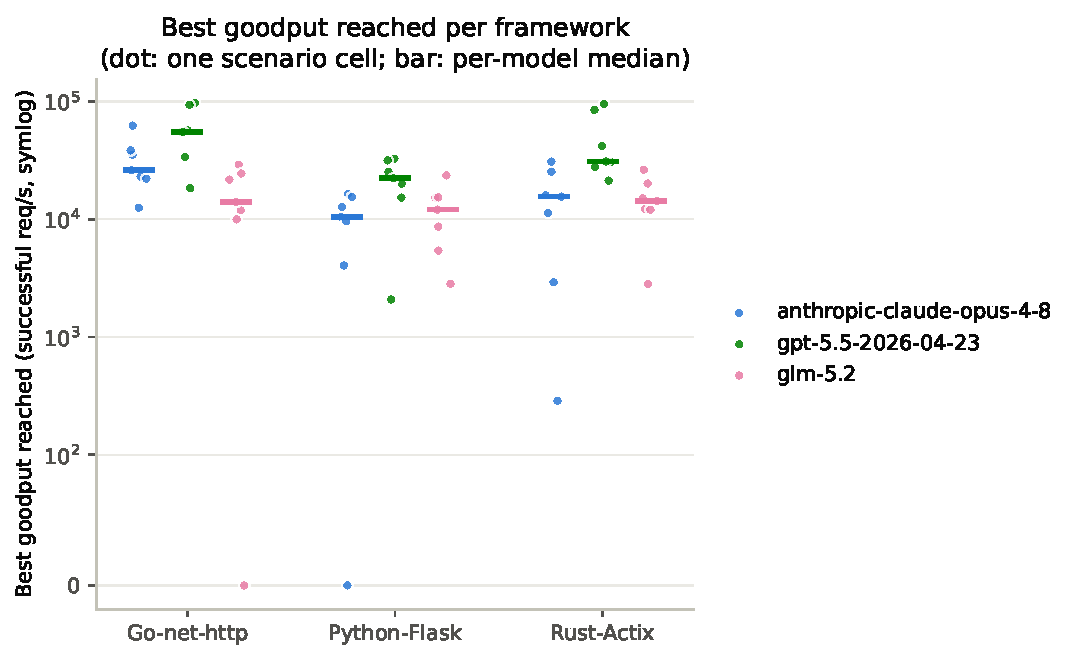
\includegraphics[width=0.85\linewidth]{figures/eval/framework_comparison.pdf}
  \caption{Best goodput reached per framework (symlog $y$-axis), split by
    model. Each dot is one scenario cell; the horizontal bar is the
    per-model geometric mean for that framework. Cells with zero goodput
    throughout are excluded from the bar, not shown at $0$.}
  \label{fig:results-framework-comparison}
\end{figure}

\paragraph{Evidence.}
Every model has seven-of-seven coverage on every framework except two
cells that never reach positive goodput (\texttt{glm-5.2}'s
\textsc{TransitPulseDelayReporter}$\times$\textsc{Go-net-http} and
\texttt{claude-opus-4-8}'s \textsc{ClickCount}$\times$\textsc{Python-Flask},
both already excluded in Section~\ref{sec:results-rq1}), so all but two of
the nine per-model framework geometric means rest on seven cells, those
two on six. \textsc{Go-net-http} reaches the highest geometric-mean
goodput for \emph{every} model: $28{,}170.1$\,req/s for
\texttt{claude-opus-4-8}, $51{,}626.2$ for \texttt{gpt-5.5}, $17{,}167.7$
for \texttt{glm-5.2}. Below that, the ordering is not consistent. For
\texttt{gpt-5.5} and \texttt{glm-5.2}, \textsc{Rust-Actix} is second
($40{,}870.9$ and $12{,}485.4$) ahead of \textsc{Python-Flask}
($16{,}749.4$ and $9{,}820.8$). For \texttt{claude-opus-4-8} the order
inverts: \textsc{Python-Flask} ($10{,}465.7$) is \emph{ahead} of
\textsc{Rust-Actix} ($7{,}847.5$), the lowest framework geometric mean for
any model in this dataset.

That inversion is not simply ``\textsc{Python-Flask} is the slow one
here'': two of \texttt{claude-opus-4-8}'s seven \textsc{Rust-Actix} cells
are exceptionally low, \textsc{Petstore} at $286.7$\,req/s and
\textsc{ClickCount} at $2{,}916.9$, both cells whose trajectory never
improves past its first success (\textsc{Petstore}$\times$\textsc{Rust-Actix}
shows the same $1.0\times$ stall for \texttt{gpt-5.5} too, at a far higher
absolute goodput of $27{,}853$\,req/s); the other five \textsc{Rust-Actix}
cells are in the same range as \texttt{claude-opus-4-8}'s other
frameworks. A geometric mean is considerably more sensitive to a couple
of low values than a median over the same seven cells, which is exactly
why this pattern did not show up under a median-based version of this
comparison.

\paragraph{Interpretation.}
\textsc{Go-net-http} setting the highest ceiling for every model is now a
clean, model-independent finding. What is model-dependent is not which
framework is \emph{best}, but which is \emph{worst}: for \texttt{gpt-5.5}
and \texttt{glm-5.2}, \textsc{Python-Flask}'s single-process WSGI ceiling
under \texttt{gunicorn} is the limiting factor; for \texttt{claude-opus-4-8},
two specific \textsc{Rust-Actix} cells that stall at their first
successful iteration pull that framework's typical performance below
\textsc{Python-Flask}'s, even though most of its \textsc{Rust-Actix}
cells are unremarkable. This is a property of the underlying data, not an
artefact of the statistic used to summarise it, but \emph{which}
statistic is used determines whether it is visible at all: a robust
central-tendency measure such as a median can hide exactly the kind of
collapse this thesis's RQ7 failure analysis is otherwise built to
surface.

\paragraph{Conclusion.}
\textbf{Framework sets an achievable-goodput ceiling that refinement
operates within, not around, and \textsc{Go-net-http} sets the highest
ceiling for every model.} Which framework sets the \emph{lowest} ceiling
is not universal: \textsc{Python-Flask} for \texttt{gpt-5.5} and
\texttt{glm-5.2}, but \textsc{Rust-Actix} for \texttt{claude-opus-4-8},
the latter driven by two cells that stall at their first successful
iteration rather than by a general weakness of that framework for this
model.


% ----- §5.7 RQ6 -----
\section{RQ6: What Deployment Parameters Does the Agent Converge To?}
\label{sec:results-rq6}

\paragraph{Evidence.}
Spec prompts intentionally omit recommended numeric ranges
(Section~\ref{sec:methods-spec}), so any sensible-looking convergence in
\texttt{backend.replicas}, per-pod resource requests, or database
topology is evidence the agent is reading load-test and utilisation
feedback rather than falling back on defaults. The clearest example
remains \texttt{gpt-5.5} on \textsc{ClickCount}$\times$\textsc{Go-net-http},
whose $75.4\times$ gain (baseline $1{,}285.1$\,req/s to best
$96{,}924.9$\,req/s) is the single largest in this dataset:

\begin{table}[htbp]
  \centering
  \caption{Spec-knob trajectory for \texttt{gpt-5.5}, \textsc{ClickCount},
    \textsc{Go-net-http} (selected iterations).}
  \label{tab:results-rq6-clickcount}
  \footnotesize
  \begin{tabular}{@{}rrrrrrr@{}}
    \toprule
    Iter.\ & Lever & Goodput (req/s) & Replicas & CPU req.\ & DB repl.\ & DB max\_conn \\
    \midrule
    000 & baseline & 1{,}285.1  & 48  & 1000m & 3 & 500 \\
    006 & code     & 23{,}670.6 & 48  & 1000m & 3 & 500 \\
    007 & spec     & 23{,}640.9 & 192 & 350m  & 1 & 300 \\
    008 & code     & 90{,}653.8 & 192 & 350m  & 1 & 300 \\
    009 & spec     & 91{,}392.6 & 320 & 250m  & 1 & 500 \\
    010 & code     & 96{,}924.9 & 320 & 250m  & 1 & 500 \\
    \bottomrule
  \end{tabular}
\end{table}

Between iterations 006 and 010, the agent roughly \emph{sextuples}
replica count (48 $\to$ 320) while \emph{quartering} per-pod CPU request
(1000m $\to$ 250m), trading a few large pods for many small ones, and
drops database replicas from 3 to 1. For a scenario whose endpoints are a
near-stateless counter increment (Section~\ref{sec:setup-scenarios}),
this is the correct qualitative direction: per-request CPU cost is
negligible, so raw horizontal fan-out beats per-pod headroom, and the
extra Postgres read replicas the baseline provisioned were never
load-bearing. \texttt{glm-5.2} shows the same qualitative direction on its
own \textsc{ClickCount}$\times$\textsc{Go-net-http} cell, one of its
largest observed gains in this dataset ($14.9\times$), though a full
knob-by-knob trajectory is not reproduced here.

Not every spec-refinement decision pays off, however:
Section~\ref{sec:results-rq7} gives a case where the stated rationale is
reasonable but the resulting deployment regresses to zero goodput, and RQ3
above shows this is not a one-off: \texttt{glm-5.2}'s spec-refinement mean
is net-negative across 66 steps, and \texttt{claude-opus-4-8}'s
\textsc{BranchWeave}$\times$\textsc{Rust-Actix} cell
(Section~\ref{sec:results-rq1}) shows the same failure mode ending a
trajectory outright rather than just dipping mid-way through it.

\paragraph{Interpretation.}
Where the agent has enough successful iterations to work with, its
\texttt{spec.yaml} trajectory tracks the workload's actual scaling
characteristics rather than converging on generic defaults, which is the
behaviour the constrained-schema design of Section~\ref{sec:methods-design}
was intended to elicit. That the two models with the largest observed
gains (\texttt{gpt-5.5} and \texttt{glm-5.2}) both reach it on the same
scenario, via qualitatively similar knob movements, is stronger evidence
than a single case study that this reflects the workload's actual scaling
shape rather than one model's idiosyncratic behaviour.

\paragraph{Conclusion.}
\textbf{The agent converges on workload-appropriate deployment parameters
when given the room to iterate}, corroborated on the same scenario by two
different models, but this chapter reports one detailed trajectory, not a
systematic per-cell audit; RQ7's counter-example, and RQ3's model-level
spec statistics, show this is a tendency, not a guarantee, and RQ1's
\textsc{BranchWeave}$\times$\textsc{Rust-Actix} cell shows the downside
case can be severe enough to end a trajectory rather than just cost it a
few iterations.


% ----- §5.8 RQ7 -----
\section{RQ7: Failure Modes and Case Studies}
\label{sec:results-rq7}

\begin{figure}[htbp]
  \centering
  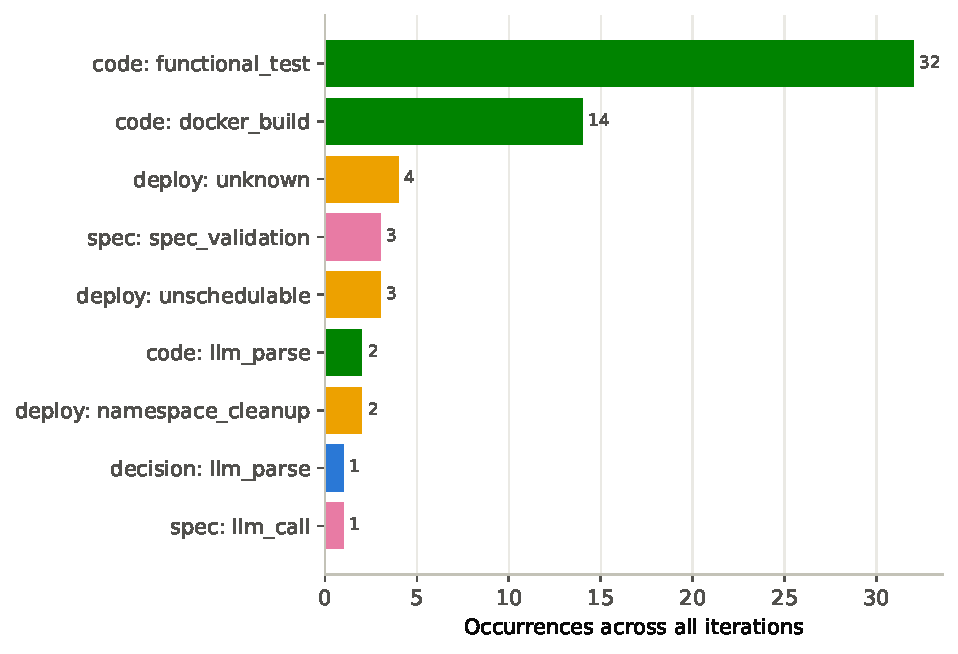
\includegraphics[width=0.75\linewidth]{figures/eval/failure_taxonomy.pdf}
  \caption{Recorded \texttt{failure.json} occurrences by phase and kind,
    summed across all three models and all 63 cells.}
  \label{fig:results-failure-taxonomy}
\end{figure}

\paragraph{Evidence.}
Of \textbf{62} recorded failures, \textbf{32} are \texttt{02-code:
functional\_test} failures, split 4 / 13 / 15 across
\texttt{claude-opus-4-8} / \texttt{gpt-5.5} / \texttt{glm-5.2}, and these
remain the dataset's largest genuine code-correctness signal.
\textbf{14} are \texttt{docker\_build} failures (Rust or Go code that fails
to compile), 12 of them \texttt{glm-5.2}'s and 2 \texttt{gpt-5.5}'s.
Together, functional-test and docker-build failures account for 46 of the
62 recorded failures (74\%). Notably, \texttt{claude-opus-4-8}'s
\textsc{BranchWeave}$\times$\textsc{Rust-Actix} cell
(Section~\ref{sec:results-rq1}) contributes \emph{zero} entries to this
count despite ending at zero goodput: every one of its ten iterations
completed as a harness-level success, so its late collapse is invisible
here and only shows up in the goodput trajectory itself, a further
illustration that this failure taxonomy tracks harness-detected problems,
not final outcome quality.

Two related deploy-phase findings share the same underlying symptom under
different labels. \texttt{claude-opus-4-8}'s
\textsc{Petstore}$\times$\textsc{Python-Flask} cell shows two
\texttt{unschedulable} failures (iterations 005--006, both spec-refinement):
a proposed spec passed static validation but its resources could not
actually be scheduled onto any node at apply time.
\texttt{glm-5.2}'s \textsc{ParcelPinLockerPickup}$\times$\textsc{Go-net-http}
cell shows the same summary text, ``Kubernetes resources did not become
Ready within timeout'', on two consecutive spec-refinement iterations
(002--003), but recorded under a different kind, \texttt{namespace\_cleanup}.
A third occurrence of the same summary text and \texttt{unschedulable} kind
appears on \texttt{glm-5.2}'s
\textsc{ParcelPinLockerPickup}$\times$\textsc{Rust-Actix} cell (iteration
004, code-phase), but its diagnostic detail shows a different underlying
cause from the other two: every backend pod is \texttt{CrashLoopBackOff}
across all four worker nodes, an application-level crash, not a
resource-scheduling shortfall. That two distinct root causes
(genuine scheduling infeasibility, and an application repeatedly crashing
after it is already scheduled) surface under the same \texttt{unschedulable}
label, and that the \emph{same} symptom text appears under two different
kind labels elsewhere, means this kind field cannot be read at face value
without checking the underlying diagnostic; it is a labelling gap worth
noting for anyone extending this taxonomy, not three independent findings
about scheduling itself.

A separate, genuinely recurring deploy-phase issue shows up for two
different models: a \texttt{docker tag failed: ... No such image} error,
recorded as kind \texttt{unknown}, on \texttt{claude-opus-4-8}'s
\textsc{Recipes}$\times$\textsc{Python-Flask} cell (iterations 005--006)
and \texttt{glm-5.2}'s \textsc{Petstore}$\times$\textsc{Rust-Actix} cell
(iterations 005--006). Both recover within a few iterations. Recurring
across two unrelated models and scenarios makes a harness-level
build/registry propagation race more likely than a model- or
scenario-specific cause, though this dataset cannot confirm that directly.

A positive counter-example is worth recording alongside the gaps above:
\texttt{claude-opus-4-8}'s \textsc{TransitPulseDelayReporter}$\times$\textsc{Go-net-http}
cell (iteration 001) shows static spec validation \emph{correctly}
rejecting a proposal before it was ever applied, pinning all three
database replicas onto one worker node whose combined resource request
(38{,}000m CPU) exceeded that node's allocatable budget
($\approx${}28{,}800m). A second instance of the same check firing
correctly appears on \texttt{glm-5.2}'s
\textsc{TransitPulseDelayReporter}$\times$\textsc{Python-Flask} cell
(iteration 002), again a database placement pinning $32{,}000$m CPU onto
one node. This is exactly the check the
\texttt{unschedulable}/\texttt{namespace\_cleanup} cases above show gaps
in, working as designed in both instances.

The remaining kinds are small in count but each a distinct, genuine
signal: \textbf{3} \texttt{spec\_validation} failures (the two node-pinning
cases just described, plus \texttt{glm-5.2}'s
\textsc{Recipes}$\times$\textsc{Rust-Actix} cell), \textbf{3}
decision- or code-phase \texttt{llm\_parse} failures (all
\texttt{glm-5.2}: \textsc{Petstore}$\times$\textsc{Go-net-http} at baseline,
and \textsc{SplitNestSharedExpenseLedger} on both
\textsc{Go-net-http}\,(iteration 006) and \textsc{Rust-Actix}\,(iteration
010)), and \textbf{1} \texttt{llm\_call} failure that is not a transport
fault: \texttt{gpt-5.5}'s \textsc{Petstore}$\times$\textsc{Python-Flask}
cell hit its own configured \texttt{--llm-max-cost} ceiling (\$20.22 spent
against a \$20.00 cap) at iteration 010, the framework's cost-tracking
safeguard (Section~\ref{sec:methods-workflow}) doing exactly what it is
designed to do.

\paragraph{Case study: a connection-pooling bug invisible to
single-container evaluation.} \texttt{glm-5.2}'s
\textsc{Recipes}$\times$\textsc{Go-net-http} baseline reaches a completed
bench but records \textbf{0} sustained goodput: the adaptive profile's
warm-up step fails health checks and explore never starts. Postgres logs
from that run show the deployment producing 953 errors during the load
window, dominated by two error classes:
\texttt{\small unnamed prepared statement does not exist} and
\texttt{\small bind message supplies N parameters, but prepared statement
requires M}. This is the classic symptom of a Go SQL driver using
server-side prepared statements against PgBouncer in \texttt{transaction}
pooling mode, where a prepared statement created on one physical
connection is invisible on the next pooled connection a later query lands
on. This bug is invisible to \textsc{BaxBench}'s original single-container
functional tests (which use a direct, unpooled connection) and only
manifests once the generated code is deployed behind the pooler this
framework introduces. Iteration~001 (code refinement) does not fix it
(goodput remains 0); iteration~002 (code refinement again, chosen freely
by the decision stage given the iteration~001 failure feedback) does,
jumping to $19{,}026.7$\,req/s. This is direct evidence that iterative
\emph{code} refinement, not deployment tuning, is the correct lever for
an infra-interaction bug the model could not have anticipated at
generation time, and that it can take more than one attempt.

\paragraph{Case study: a plausible deployment decision that backfires.}
On the same cell, iteration~003's decision stage reasons as follows
(quoted verbatim from its \texttt{decision.json}):
\begin{quote}
\small
``The code is now well-optimized (0\% failures, 19K/s goodput) and the
bottleneck is purely infrastructure: Postgres hits 200/200 connections
with PgBouncer \texttt{cl\_waiting} reaching 311, and db-primary CPU
saturates at 16.7 cores. [...] We should add database replicas, enable a
read pooler, increase Postgres \texttt{max\_connections} and PgBouncer
\texttt{default\_pool\_size}, and potentially reduce over-provisioned
backend CPU to free cluster budget for more DB resources.''
\end{quote}
The reasoning is a coherent read of the previous iteration's diagnostics
(Section~\ref{sec:methods-bench}), and the resulting spec does exactly
what it describes: database replicas 1 $\to$ 3, \texttt{max\_connections}
200 $\to$ 300, backend CPU request 2000m $\to$ 500m. The resulting
deployment, however, regresses to \textbf{0} sustained goodput. The next
iteration (004, code) recovers to $20{,}494.3$\,req/s \emph{without}
reverting the topology change, so the regression is not explained by the
added replicas alone; most plausibly the simultaneous $4\times$ backend
CPU cut left the application under-provisioned for its own request
handling while the new DB topology was still stabilising. The cell goes
on to alternate lever choices through the rest of its budget, peaking at
$24{,}477.3$\,req/s at iteration~007 before settling at $21{,}722.2$\,req/s
by iteration~010, itself not a monotonic climb, with two further
consecutive code-refinement steps (iterations~008--009) that give back
part of the gain before the final spec step recovers it. Unlike
\texttt{claude-opus-4-8}'s \textsc{BranchWeave}$\times$\textsc{Rust-Actix}
cell (Section~\ref{sec:results-rq1}), this trajectory has enough budget
left after its own backfire to recover before running out.
\textbf{Lesson for the framework, not just the model}: this iteration
changed three spec fields at once, which is consistent with the
single-lever-per-iteration design (Section~\ref{sec:methods-workflow}) but
does not prevent \emph{multiple fields within one lever} from changing
simultaneously, which limits attribution within a spec-refinement step the
same way mixing code and spec changes would across steps. RQ3's finding
that \texttt{glm-5.2}'s spec-refinement mean is net-negative across 66
steps suggests this is not a one-off either for this cell or this model.

\paragraph{Interpretation.}
The evidence supports a consistent reading: essentially all \emph{genuine}
attrition happens at the code-correctness gate the agent is directly
responsible for (functional-test and docker-build failures together
account for 46 of 62 recorded failures), and the cluster-execution path is
close to, but not quite, failure-free. The two case studies together show
the same lesson from opposite directions: code refinement can fix bugs the
model could not have anticipated (the pooling case), and a single
deployment decision can undo a healthy deployment even when its diagnosis
is correct, because the framework does not constrain how many fields one
spec-refinement step may touch (the backfire case). The
\texttt{unschedulable}/\texttt{namespace\_cleanup} labelling gap is a
finding about the evaluation framework's own failure taxonomy rather than
about any model, and RQ1's \textsc{BranchWeave}$\times$\textsc{Rust-Actix}
cell shows that this failure record is blind to a genuinely important
outcome: a trajectory can end at zero goodput without a single entry
appearing here.

\paragraph{Conclusion.}
\textbf{The dominant \emph{genuine} failure mode is upstream of
deployment}, in code correctness (functional-test and docker-build
failures together are 74\% of recorded failures). The cluster-execution
path is nearly, not entirely, failure-free: the
\texttt{unschedulable}/\texttt{namespace\_cleanup} cases point at a real
gap between static validation and actual scheduling feasibility, and at a
labelling inconsistency in how that gap is recorded, partially offset by
two documented cases where the same static validation correctly caught an
infeasible proposal before it was ever applied. A separate gap, not in
scheduling but in reporting, is that this failure taxonomy does not
capture a trajectory ending at zero goodput when every individual
iteration is a harness-level success.


% ----- §5.9 Cross-Cutting Synthesis -----
\section{Cross-Cutting Synthesis}
\label{sec:results-synthesis}

Read together across all 63 cells, three models, and seven scenarios, four
patterns recur consistently enough to generalise beyond any single cell:

\begin{itemize}
  \item \textbf{Correctness gates deployment, consistently.} The largest
        single source of attrition (RQ7, 74\% of recorded failures) and
        the largest single-step goodput gains (RQ3) both trace back to
        code correctness, not deployment tuning. This holds across every
        model and is exactly the class of bug BaxBench's original
        single-container evaluation cannot observe
        (Section~\ref{sec:rw-benchmarks}).
  \item \textbf{Deployment refinement is real, bounded, and carries a
        downside risk that is not exclusive to one model.} Across every
        model, spec refinement's median per-step effect is small; its
        mean is now the smaller of the two levers for every model (RQ3),
        sharply negative for \texttt{glm-5.2} and, in one new
        \texttt{claude-opus-4-8} cell, severe enough to end a trajectory
        at zero goodput outright (RQ1, RQ7).
  \item \textbf{The three models are equally reliable but not equally
        capable or costly.} Every model completes its full budget on
        100\% of its 21 cells, so the meaningful comparison is achieved
        goodput against cost: \texttt{gpt-5.5} reaches roughly double the
        geometric-mean goodput of the other two without costing
        proportionally more, while \texttt{glm-5.2} matches
        \texttt{claude-opus-4-8}'s goodput at under a fifth of its cost
        (RQ4). \textsc{Go-net-http} sets the highest ceiling for every
        model, while which framework sets the \emph{lowest} is
        model-dependent: \textsc{Python-Flask} for \texttt{gpt-5.5} and
        \texttt{glm-5.2}, but \textsc{Rust-Actix} for
        \texttt{claude-opus-4-8} (RQ5).
  \item \textbf{The cluster-execution path is close to, but not quite, a
        failure-free component, and the failure taxonomy itself has
        blind spots.} Deploy-phase failures remain a small fraction of the
        total (RQ7), and the same static validation that occasionally
        misses a scheduling infeasibility also demonstrably catches it,
        twice, in the node-over-commit cases documented in
        Section~\ref{sec:results-rq7}; separately, a trajectory that ends
        at zero goodput through two ordinary-looking spec decisions
        generates no failure record at all.
\end{itemize}


% ----- §5.10 Summary -----
\section{Summary}
\label{sec:results-summary}

Across all three models and all 63 scenario/framework cells:
%
\begin{itemize}
  \item iterative refinement improves sustained goodput in essentially
        every cell, and separately rescues 27 of the 29 \emph{dead}
        baselines observed into a working deployment; one further cell,
        healthy at baseline, climbs well above it and then loses
        everything again at the very end of its budget (RQ1);
  \item code refinement contributes the largest single-step gains for
        all three models and now exceeds deployment refinement's mean for
        all three as well, dominated by fixes to bugs that only manifest
        under load and cluster topology; deployment refinement is smaller
        on median for all three, positive on average for two of three,
        and net-negative for \texttt{glm-5.2} (RQ3);
  \item \textbf{all three models complete every cell}, so the meaningful
        comparison is achieved goodput against cost: \texttt{gpt-5.5}
        reaches the highest absolute goodput without costing
        proportionally more, while \texttt{glm-5.2} matches
        \texttt{claude-opus-4-8}'s goodput at under a fifth of the cost
        (RQ4);
  \item \textsc{Go-net-http} sets the highest achievable-goodput ceiling
        for all three models; which framework sets the \emph{lowest} is
        not universal (\textsc{Python-Flask} for \texttt{gpt-5.5} and
        \texttt{glm-5.2}, but \textsc{Rust-Actix} for
        \texttt{claude-opus-4-8}) (RQ5);
  \item where it converges, the agent's deployment-spec trajectory tracks
        workload characteristics sensibly, corroborated across two models
        on the same scenario (RQ6), though not every individual
        spec-refinement decision improves the outcome, even when the
        stated rationale is sound, and in one case the downside is severe
        enough to end the trajectory (RQ7);
  \item nearly all \emph{genuine} attrition happens at the
        code-correctness gate the agent is responsible for; the
        cluster-execution path is nearly, not entirely, failure-free, and
        the failure taxonomy itself has a blind spot for trajectories that
        end at zero goodput without a harness-level failure (RQ7).
\end{itemize}

These findings are discussed further, including limitations and threats
to validity, in Chapter~\ref{ch:discussion}, and answered directly against
the thesis's research question in Chapter~\ref{ch:conclusion}.
